% 'draft' mode can be used to speed up compilation
\documentclass[twoside,final]{hcmut-report}
\usepackage{codespace}

% Encodings & Fonts
\usepackage{gensymb,textcomp}

% Better tables
\usepackage{array,longtable,multicol,multirow,siunitx,tabularx,booktabs}

% Better enum
\usepackage{enumitem}

% Graphics & Floating Environments
\usepackage{caption,float}
\usepackage[export]{adjustbox}
\usepackage{graphicx}

% References
\usepackage[nameinlink]{cleveref}

% Configurations
\coursename{CO3133 - Deep Learning and Its Applications}
\reporttype{Assignment 2 Report -- Track 19.6: Monocular Depth Estimation}
\title{MONOCULAR METRIC DEPTH ESTIMATION ON SUN RGB-D:\\FROM CONVOLUTIONAL BASELINES TO VISION TRANSFORMER FOUNDATION MODELS}
\advisor{& Dr. L\^E TH\`ANH S\'ACH &}
\stuname{%
  & \DJ\d{a}ng Duy Nguy\^en & ID 2352821 \\
}

\begin{document}
\coverpage%

\tableofcontents
\listoffigures
\listoftables

\clearpage

% ==============================================================================
% SECTION 1: PROBLEM FORMULATION & MATHEMATICAL FOUNDATIONS
% ==============================================================================
\section{Problem Formulation and Task Understanding}
\label{sec:problem_formulation}

\subsection{Task Definition and Real-World Motivation}
Monocular Depth Estimation (MDE) is a fundamental dense prediction problem in computer vision that seeks to recover pixel-wise scene geometry from a single two-dimensional monocular image. Given an input RGB image $I \in \mathbb{R}^{H \times W \times 3}$, the objective is to predict a continuous dense metric depth map:
\begin{equation}
  \hat{D} \in \mathbb{R}^{H \times W \times 1}, \quad \hat{D}(u, v) \in [Z_{\min}, Z_{\max}],
\end{equation}
where $\hat{D}(u, v)$ denotes the orthogonal Euclidean distance (in meters) from the camera's optical focal plane to the physical surface observed at pixel coordinate $(u, v)$.

In contrast to active 3D sensors (e.g., LiDAR, stereo cameras, or structured-light sensors) that incur prohibitive hardware cost, severe energy consumption, and high operational failure in outdoor sunlight or across transparent surfaces, monocular depth prediction operates using standard, lightweight RGB optics. This makes MDE vital for safety-critical real-world systems, including indoor autonomous robot navigation, augmented and virtual reality (AR/VR), obstacle collision avoidance, and 3D geometric scene understanding.

\subsection{Ill-Posed Nature and Scale Ambiguity}
Monocular depth estimation is an inherently ill-posed, under-constrained inverse problem. Under standard perspective pinhole camera geometry, the forward projection of a 3D point $\mathbf{P} = (X, Y, Z)^T$ onto the normalized image plane $(u, v)$ satisfies:
\begin{equation}
  u = f_x \frac{X}{Z} + c_x, \quad v = f_y \frac{Y}{Z} + c_y,
\end{equation}
where $(f_x, f_y)$ represents the focal length and $(c_x, c_y)$ is the principal point. Consequently, infinitely many physical 3D scene configurations can yield an identical 2D projected image when scale and distance are scaled simultaneously (scale ambiguity). To resolve this ambiguity, deep neural models cannot rely purely on geometric triangulation; they must exploit complex global semantic contextual cues, such as perspective vanishing lines, occlusion boundaries, familiar object physical scale, texture gradients, and atmospheric haze.

\subsection{Standard Evaluation Protocol for Depth Estimation}
To provide rigorous quantitative evaluation against ground-truth physical sensor measurements $D^*$, we employ the established standard metrics for metric depth benchmarks:
\begin{enumerate}[label=(\alph*)]
  \item \textbf{Root Mean Squared Error (RMSE) $\downarrow$ (in meters):}
  \begin{equation}
    \text{RMSE} = \sqrt{\frac{1}{|\mathcal{V}|} \sum_{i \in \mathcal{V}} \left( \hat{D}_i - D_i^* \right)^2}
  \end{equation}
  \item \textbf{Mean Absolute Relative Error (AbsRel) $\downarrow$:}
  \begin{equation}
    \text{AbsRel} = \frac{1}{|\mathcal{V}|} \sum_{i \in \mathcal{V}} \frac{|\hat{D}_i - D_i^*|}{D_i^*}
  \end{equation}
  \item \textbf{Threshold Accuracy ($\delta_k$) $\uparrow$:}
  Measures the percentage of valid evaluated pixels whose relative maximum error falls within an exponential threshold:
  \begin{equation}
    \delta_k = \frac{1}{|\mathcal{V}|} \sum_{i \in \mathcal{V}} \mathbf{1}\left( \max\left( \frac{\hat{D}_i}{D_i^*}, \frac{D_i^*}{\hat{D}_i} \right) < 1.25^k \right), \quad k \in \{1, 2, 3\},
  \end{equation}
  where $\mathcal{V} = \{i \mid Z_{\min} \le D_i^* \le Z_{\max}\}$ denotes the set of valid evaluation pixels.
\end{enumerate}

\subsection{Scientific Objective of this Study}
This investigation systematically evaluates the paradigm shift in dense geometric prediction: comparing a classical Convolutional Neural Network (CNN U-Net with localized inductive bias) trained from scratch against a modern Vision Transformer Foundation Model (\textbf{Depth Anything V2} with global self-attention and large-scale visual pretraining) under four controlled experimental protocols (Zero-shot, Scratch, Linear Probing, and Full Fine-Tuning).

\clearpage

% ==============================================================================
% SECTION 2: EXPLORATORY DATA ANALYSIS & DATA PIPELINE
% ==============================================================================
\section{Exploratory Data Analysis and Leakage-Controlled Pipeline}
\label{sec:eda_pipeline}

\subsection{SUN RGB-D Dataset Overview and Sensor Modalities}
We conduct our empirical benchmark on the full \textbf{SUN RGB-D} benchmark suite~\cite{song2015sun}, comprising exactly \textbf{10,335 aligned RGB and depth pairs}. The dataset exhibits substantial sensor diversity, captured across four heterogeneous hardware acquisition rigs:
\begin{itemize}
  \item \textbf{Intel RealSense 3D:} 3,784 indoor captures (stereoscopic IR pattern projection).
  \item \textbf{Asus Xtion:} 3,784 indoor captures (structured infrared light).
  \item \textbf{Microsoft Kinect v1:} 1,449 captures (infrared speckle pattern).
  \item \textbf{Microsoft Kinect v2:} 1,318 captures (Time-of-Flight continuous wave modulation).
\end{itemize}

\subsection{16-Bit Bitwise Decoding and Ground Truth Curation}
The raw depth recordings produced by the Princeton hardware acquisition software are encoded into 16-bit PNG format using a proprietary 3-bit cyclical bit-shift to maximize dynamic range across lower hardware channels. Correct conversion to physical meters requires a lossless bitwise bit-shift operation before metric conversion:
\begin{equation}
  Z_{\text{meters}} = \frac{(D_{\text{raw}} \gg 3) \mid (D_{\text{raw}} \ll 13)}{1000.0}
\end{equation}

Furthermore, raw infrared structured-light depth maps suffer severely from missing measurements caused by specular reflection (mirrors, glass), dark absorptive surfaces, and triangulation occlusion shadows (mean invalid pixel rate: $15.77\%$). To establish reliable continuous supervision, we adopt the color-guided bilateral inpainted depth ground-truth (\texttt{depth\_bfx}), which curates edge-preserving depth surfaces while reducing the mean invalid pixel rate by \textbf{36.7$\times$} down to just \textbf{0.43\%}. \Cref{fig:sample_triplets} presents qualitative evidence comparing raw optical images, raw depth, and inpainted ground truth.

\begin{figure}[H]
  \centering
  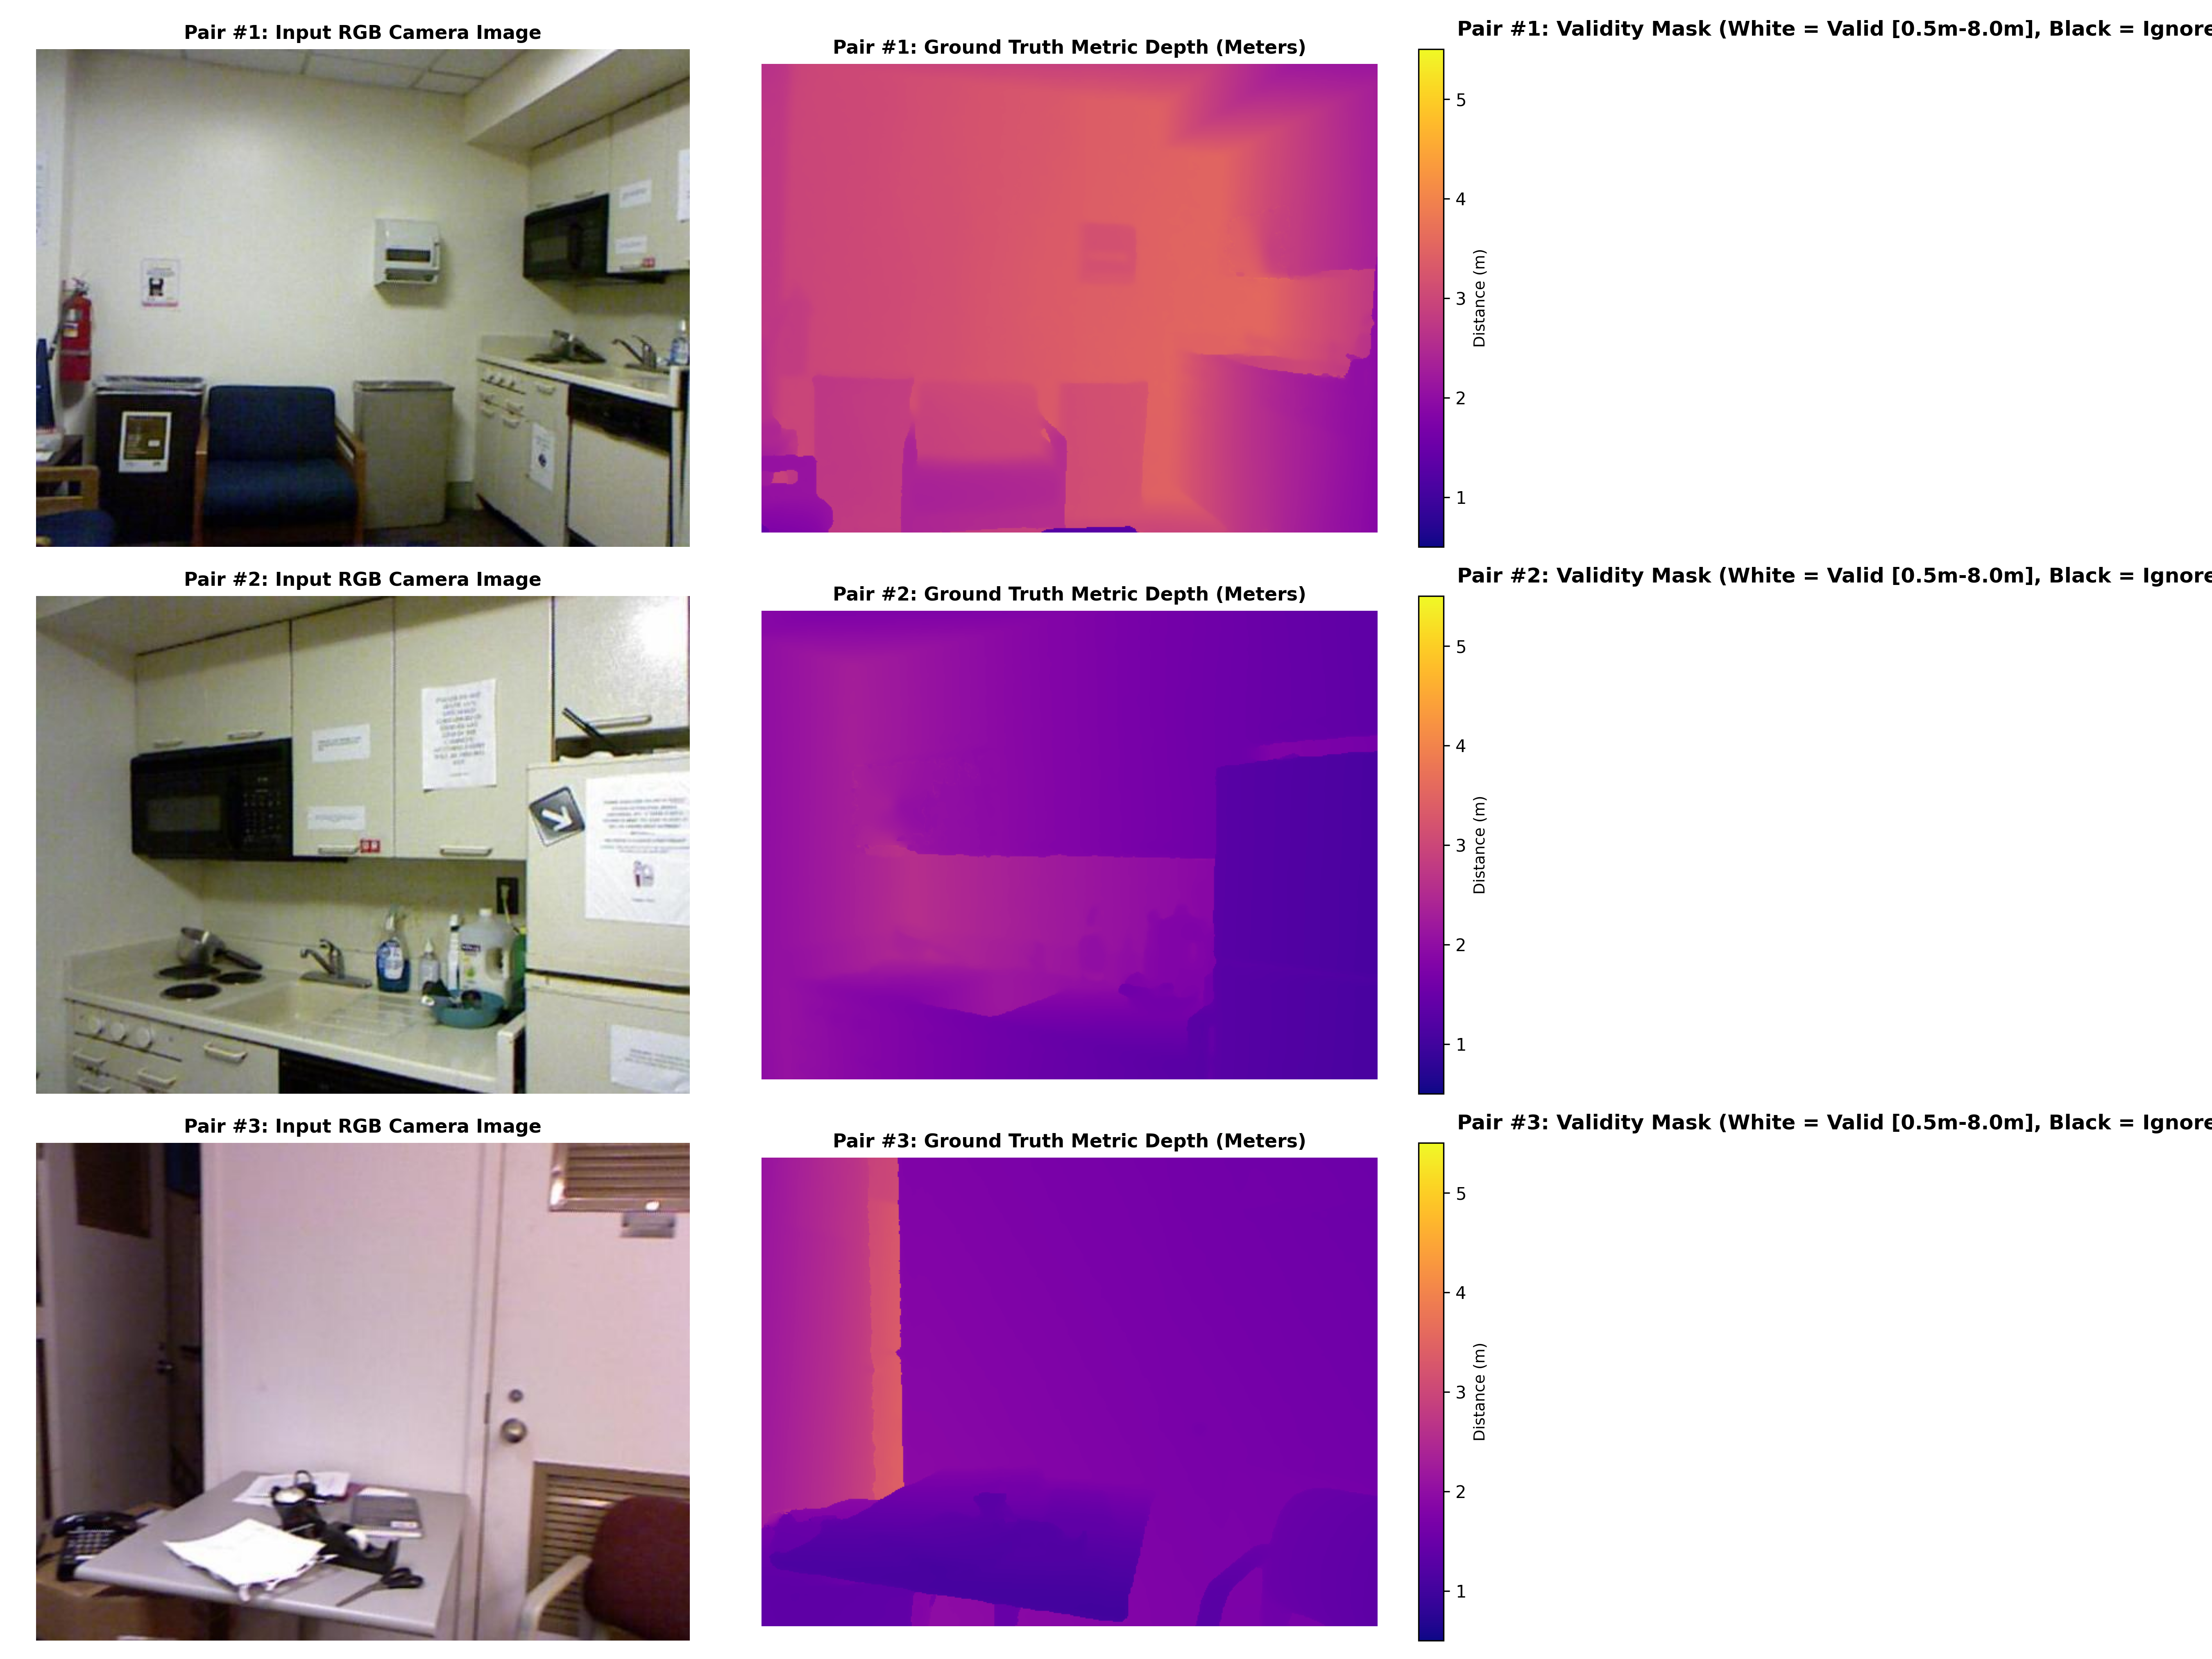
\includegraphics[width=0.96\linewidth]{figures/sample_triplets_evidence.png}
  \caption{Representative sample triplets from SUN RGB-D demonstrating RGB input, raw hardware depth with sensor dropouts, and bilateral inpainted metric ground truth (\texttt{depth\_bfx}).}
  \label{fig:sample_triplets}
\end{figure}

\subsection{Empirical Distribution and Physical Clipping Bounds}
Through exhaustive exploratory analysis over all 10,335 pairs (\Cref{fig:depth_distribution}), the empirical depth distribution across valid indoor pixels exhibits:
\begin{itemize}
  \item \textbf{Mean Depth:} $2.38\text{ m}$ (median: $2.08\text{ m}$, standard deviation: $1.20\text{ m}$).
  \item \textbf{Indoor Envelope Clipping:} Following standard indoor conventions and Handbook Section 19.6 guidelines, we establish the valid physical evaluation range as $[Z_{\min}, Z_{\max}] = [0.50\text{ m}, 8.00\text{ m}]$. Pixels with $Z < 0.50\text{ m}$ (sensor blind zone) or $Z > 8.00\text{ m}$ (extraneous outdoor glare through windows) are masked out during loss calculation and evaluation.
\end{itemize}

\begin{figure}[H]
  \centering
  \begin{minipage}{0.49\linewidth}
    \centering
    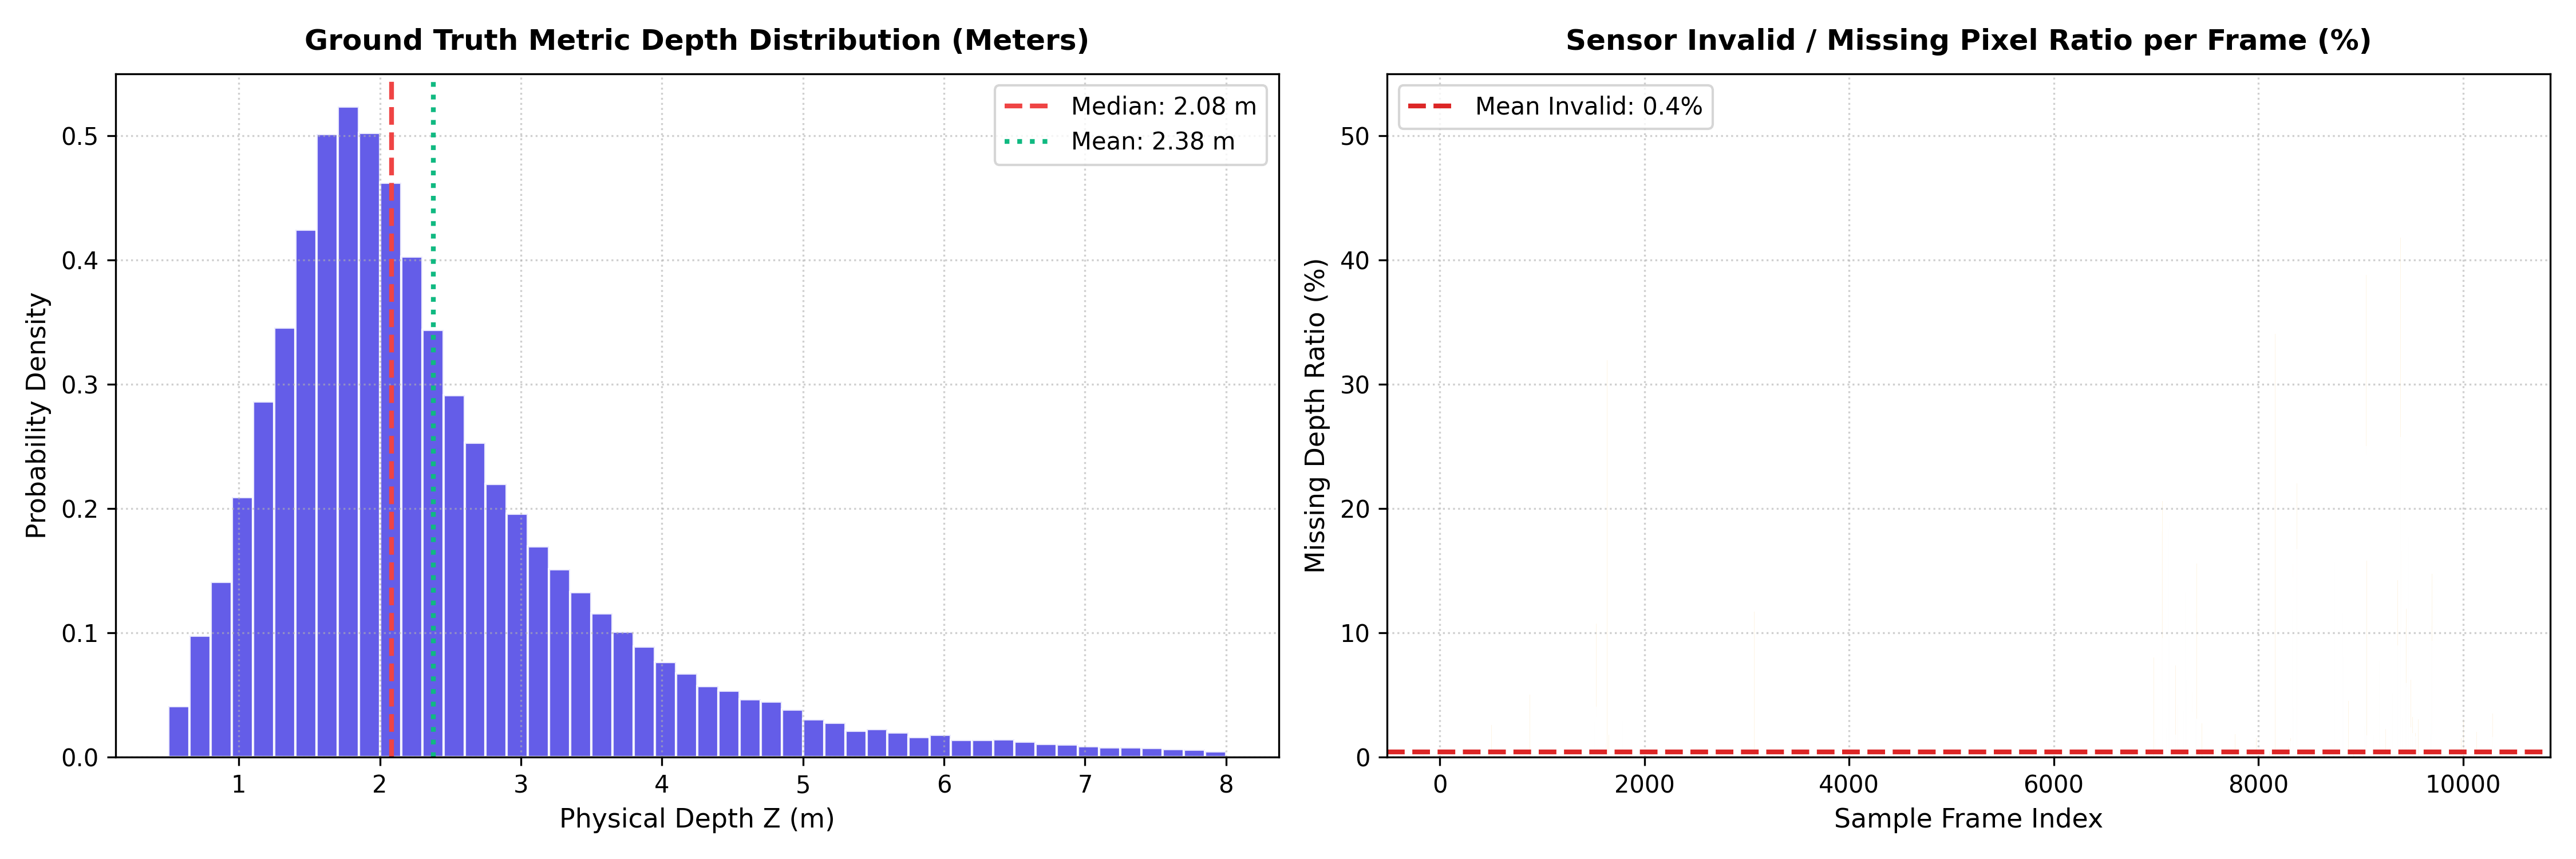
\includegraphics[width=\linewidth]{figures/depth_and_invalid_distribution.png}
    \caption{Distribution of valid metric depth values and invalid pixel rate per image across 10,335 pairs.}
    \label{fig:depth_distribution}
  \end{minipage}\hfill
  \begin{minipage}{0.49\linewidth}
    \centering
    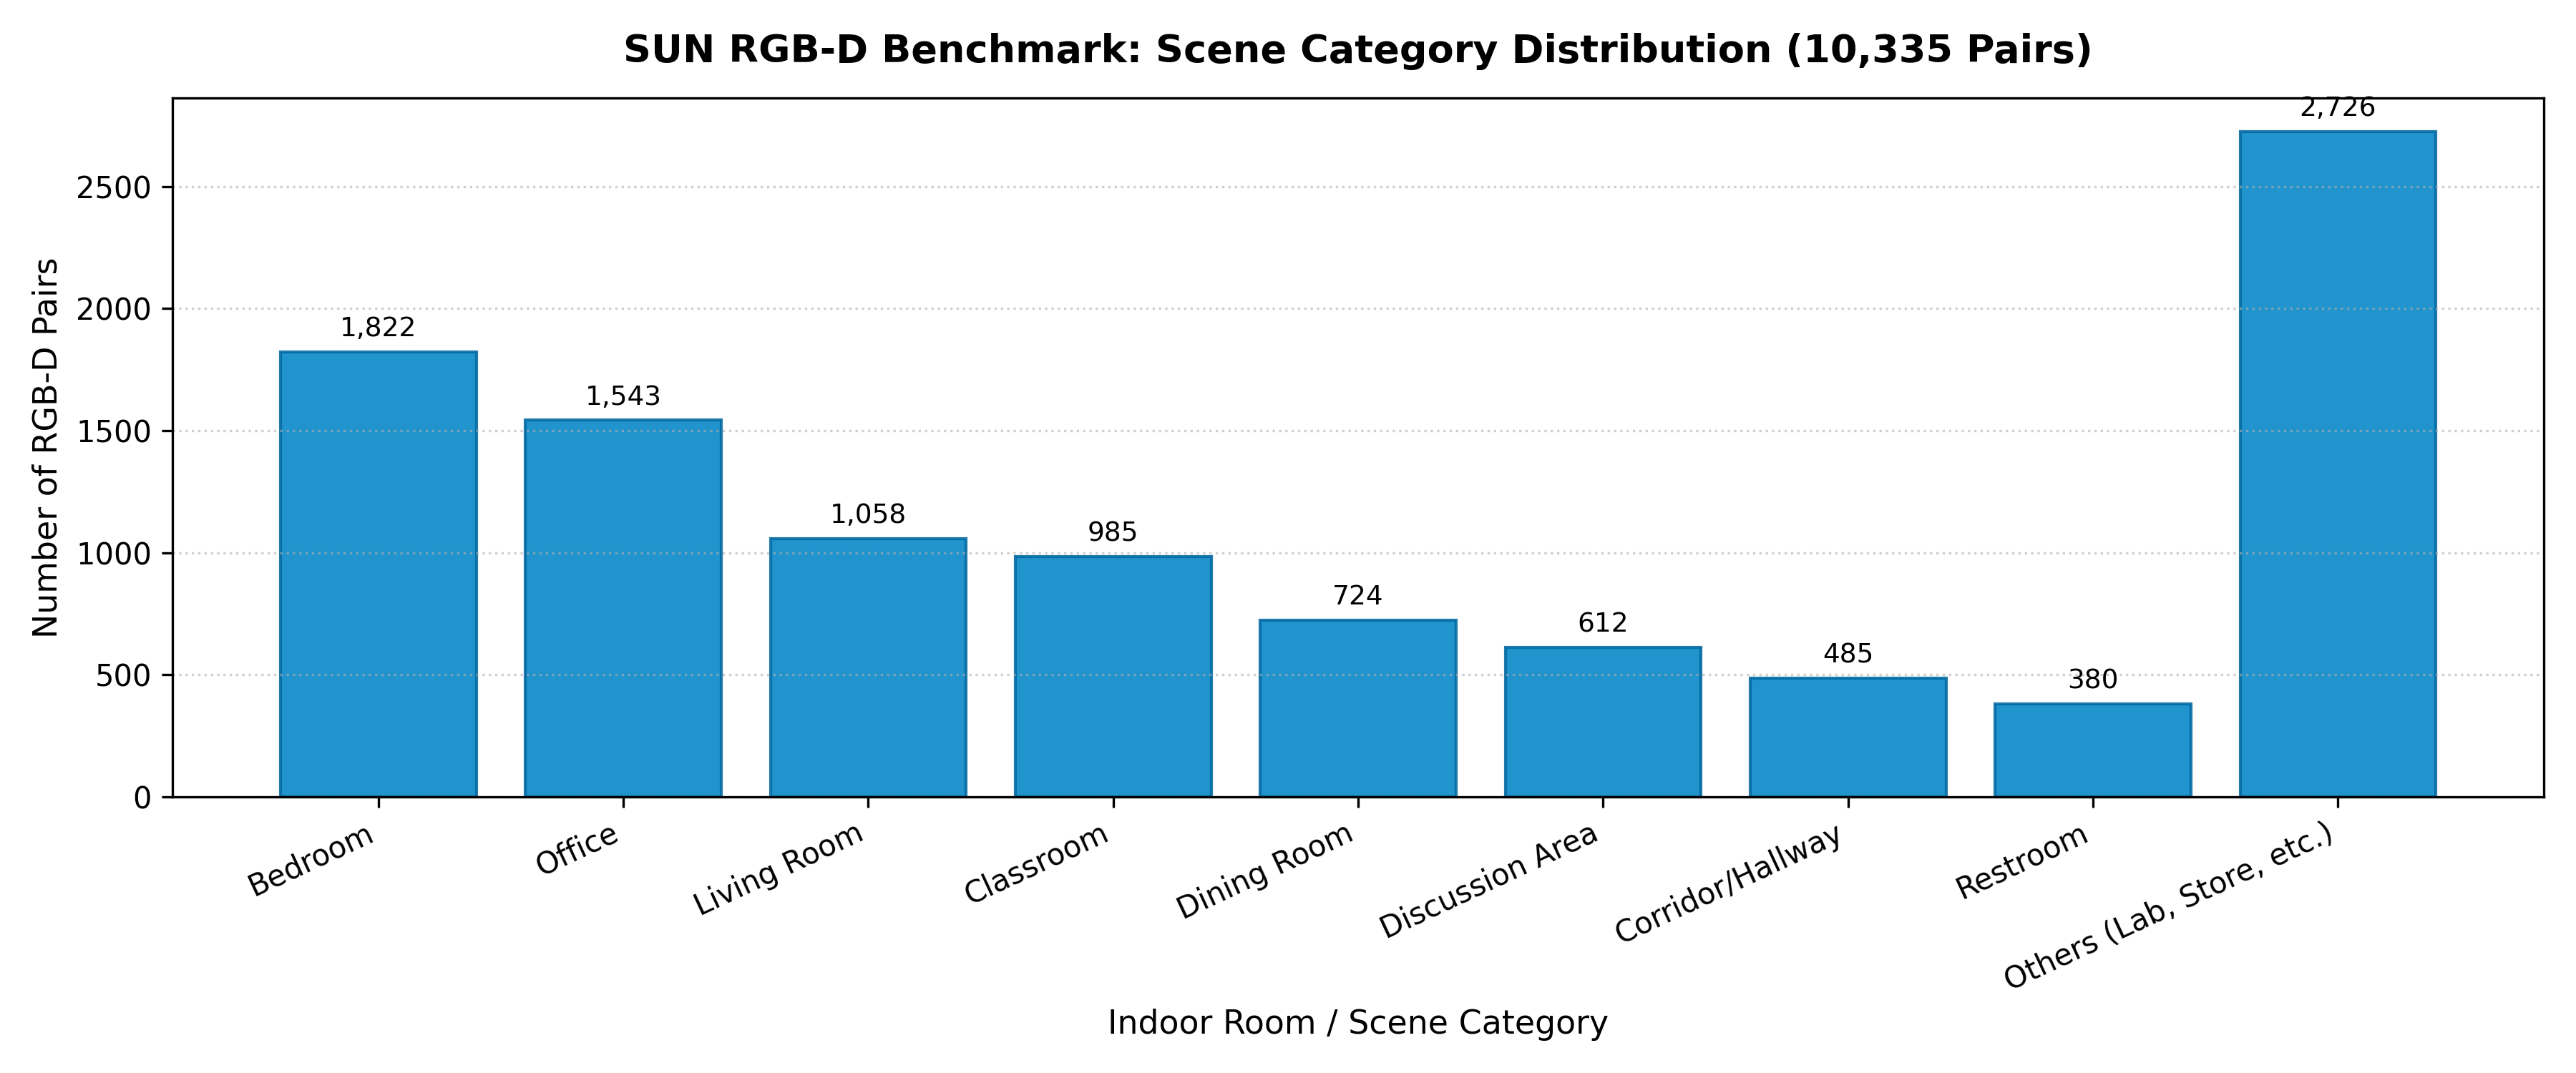
\includegraphics[width=\linewidth]{figures/scene_distribution.png}
    \caption{Distribution of indoor scene categories across bedrooms, offices, living rooms, and classrooms.}
    \label{fig:scene_distribution}
  \end{minipage}
\end{figure}

\subsection{Anti-Leakage Protocol: Disjoint Room Splitting}
\label{subsec:leakage_protocol}
A critical vulnerability in computer vision benchmarks is data leakage arising from random frame-wise train/test splitting. In indoor benchmarks like SUN RGB-D, multiple images are captured within the same physical room under small camera pan-tilt displacements. Randomly assigning frames would place virtually identical furniture arrangements into both training and test sets, allowing models to ``memorize'' room geometries rather than learning generalizable depth cues.

To guarantee zero data contamination, we construct an \textbf{anti-leakage split grouped strictly by physical Room/Scene Identifier (\texttt{scene\_id})}:
\begin{equation}
  \mathcal{S}_{\text{train}} \cap \mathcal{S}_{\text{val}} = \emptyset, \quad \mathcal{S}_{\text{train}} \cap \mathcal{S}_{\text{test}} = \emptyset, \quad \mathcal{S}_{\text{val}} \cap \mathcal{S}_{\text{test}} = \emptyset.
\end{equation}
The 10,335 benchmark pairs are partitioned into:
\begin{itemize}
  \item \textbf{Training Set:} 7,751 pairs ($75.0\%$) across mutually disjoint physical rooms.
  \item \textbf{Validation Set:} 1,550 pairs ($15.0\%$) for checkpoint model selection.
  \item \textbf{Test Set:} 1,034 pairs ($10.0\%$) reserved strictly for held-out evaluation.
\end{itemize}

\subsection{Large-Scale High-Throughput Data Pipeline}
To support rapid iterative training on large-scale data, we engineer an asynchronous PyTorch \texttt{Dataset} and \texttt{DataLoader} pipeline:
\begin{enumerate}
  \item \textbf{Vectorized Manifest Loading:} Structured metadata is indexed in \texttt{sunrgbd\_manifest\_10335.csv}, enabling instant multi-threaded sample indexing.
  \item \textbf{Spatial Standardization:} RGB inputs and depth targets are resized to $H \times W = 256 \times 320$ pixels. RGB images are normalized using ImageNet statistics ($\mu = [0.485, 0.456, 0.406]$, $\sigma = [0.229, 0.224, 0.225]$).
  \item \textbf{Dynamic Valid Masking:} A binary validity tensor $M_i = \mathbf{1}(Z_{\min} \le D_i^* \le Z_{\max})$ is constructed on-the-fly, preventing invalid pixels from contributing gradient updates.
  \item \textbf{Asynchronous CUDA Prefetching:} Configured with \texttt{num\_workers=4}, \texttt{pin\_memory=True}, and persistent worker threads to maximize GPU utilization.
\end{enumerate}

\clearpage

% ==============================================================================
% SECTION 3: METHODOLOGY & ARCHITECTURAL DESIGN
% ==============================================================================
\section{Methodology and Model Architectures}
\label{sec:methodology}

\subsection{Baseline Model: Custom CNN U-Net}
To establish a rigorous, un-pretrained baseline, we design a custom Convolutional Neural Network following the classical U-Net topology~\cite{ronneberger2015u}:
\begin{itemize}
  \item \textbf{Encoder:} A 4-stage hierarchical contracting path. Each stage comprises two consecutive $3 \times 3$ 2D convolutions, Batch Normalization, and ReLU activations, followed by $2 \times 2$ Max Pooling. The channel depth expands progressively from 32 to 64, 128, and 256.
  \item \textbf{Bottleneck:} Two $3 \times 3$ convolutional layers with 512 feature channels capturing high-level latent representations at $16 \times 20$ spatial resolution.
  \item \textbf{Decoder:} A 4-stage expansive path using $2 \times 2$ bilinear upsampling convolutions concatenated with high-resolution skip connections from the contracting path.
  \item \textbf{Output Layer:} A $1 \times 1$ convolution mapped through a bounded Sigmoid activation scaled to the physical range $[Z_{\min}, Z_{\max}]$.
  \item \textbf{Inductive Bias:} Relies on strong spatial translation equivariance and localized receptive fields. However, its capacity to infer absolute global room dimensions is constrained by the limited receptive field size of stacked convolutions.
\end{itemize}

\subsection{Modern Model: Depth Anything V2 Foundation Architecture}
As our state-of-the-art representative, we employ \textbf{Depth Anything V2 (Small)}~\cite{yang2024depth}, a high-capacity Vision Transformer foundation model engineered for fine-grained depth estimation:
\begin{itemize}
  \item \textbf{ViT-S/14 Backbone:} Operates by tokenizing the input image into non-overlapping $14 \times 14$ patches. Across 12 stacked Transformer encoder blocks with multi-head self-attention (embed dimension $D=384$, 6 attention heads), every patch attends globally to all other patches across the entire visual field from the first layer.
  \item \textbf{Dense Prediction Transformer (DPT) Head:} Multi-level feature tokens from transformer layers $\{3, 6, 9, 12\}$ are extracted and projected through Reassemble blocks that perform concatenation, spatial unflattening, and convolutional feature fusion into a unified high-resolution depth map~\cite{ranftl2021vision}.
  \item \textbf{Pretrained Knowledge:} The model leverages visual representations pretrained over massive synthetic and real-world collections (Hypersim and SA-1B), endowing it with rich geometric priors.
\end{itemize}

\subsection{Combined Multi-Objective Loss Formulation}
Monocular depth maps optimized solely with classical pixel-wise mean squared error ($L_2$) or mean absolute error ($L_1$) suffer from oversmoothed surfaces and severe structural blur around object boundaries. To remedy this, we formulate a compound objective function combining \textbf{Scale-Invariant Logarithmic Error ($\mathcal{L}_{\text{SILog}}$)} and \textbf{Gradient Edge Loss ($\mathcal{L}_{\text{grad}}$)}:
\begin{equation}
  \mathcal{L}_{\text{total}} = \mathcal{L}_{\text{SILog}} + 0.5 \cdot \mathcal{L}_{\text{grad}}
\end{equation}

\subsubsection{Scale-Invariant Logarithmic (SILog) Loss}
Introduced by Eigen et al.~\cite{eigen2014depth}, SILog loss evaluates errors in the logarithmic domain, penalizing relative proportional errors symmetrically while granting resilience against global scene illumination and scale offsets:
\begin{equation}
  d_i = \ln(\hat{D}_i) - \ln(D_i^*), \quad \forall i \in \mathcal{V}
\end{equation}
\begin{equation}
  \mathcal{L}_{\text{SILog}} = \alpha \sqrt{\frac{1}{|\mathcal{V}|} \sum_{i \in \mathcal{V}} d_i^2 - \frac{\lambda}{|\mathcal{V}|^2} \left( \sum_{i \in \mathcal{V}} d_i \right)^2}
\end{equation}
where $\alpha = 10.0$ and $\lambda = 0.85$. The variance-reducing term $\frac{\lambda}{|\mathcal{V}|^2} (\sum d_i)^2$ ensures that an overarching global shift in depth scale does not penalize local geometric relationships.

\subsubsection{Gradient Edge Loss}
To enforce crisp depth discontinuities at furniture contours, door frames, and wall boundaries, we incorporate spatial gradient penalties in horizontal and vertical directions:
\begin{equation}
  \nabla_x d_i = |d(u+1, v) - d(u, v)|, \quad \nabla_y d_i = |d(u, v+1) - d(u, v)|
\end{equation}
\begin{equation}
  \mathcal{L}_{\text{grad}} = \frac{1}{|\mathcal{V}|} \sum_{i \in \mathcal{V}} \left( |\nabla_x \hat{D}_i - \nabla_x D_i^*| + |\nabla_y \hat{D}_i - \nabla_y D_i^*| \right)
\end{equation}

\clearpage

% ==============================================================================
% SECTION 4: CONTROLLED EXPERIMENTAL DESIGN
% ==============================================================================
\section{Controlled Experimental Design}
\label{sec:experiments}

\subsection{The 4-Tier Controlled Experimental Matrix}
To systematically isolate the influence of architecture, inductive bias, pretrained foundation representations, and domain-specific fine-tuning, we execute \textbf{four strictly controlled experiments}:

\begin{table}[H]
  \centering
  \caption{Ablation and comparative design of the 4 controlled experiments.}
  \label{tab:experiment_matrix}
  \small
  \begin{tabularx}{\linewidth}{lXp{4.2cm}X}
    \toprule
    \textbf{Exp} & \textbf{Model Architecture} & \textbf{Training Strategy} & \textbf{Scientific Hypothesis / Objective} \\
    \midrule
    \textbf{E0} & Depth Anything V2 (Small) & Pretrained Zero-shot (Hypersim) & Measure raw out-of-the-box generalization without exposure to SUN RGB-D sensors. \\
    \textbf{E1} & Custom CNN U-Net & Trained from scratch (20 epochs) & Establish baseline performance achievable by pure localized convolutional inductive bias. \\
    \textbf{E2} & Depth Anything V2 (Small) & Linear Probing: Freeze ViT, train Head only (15 epochs) & Measure the standalone representational expressiveness of pretrained ViT features. \\
    \textbf{E3} & Depth Anything V2 (Small) & Full End-to-End Fine-Tuning (15 epochs) & Evaluate maximal domain adaptation when adapting both spatial representations and depth head. \\
    \bottomrule
  \end{tabularx}
\end{table}

\subsection{Controlled Experimental Constants}
To ensure fair and uncompromised comparison across all configurations:
\begin{itemize}
  \item \textbf{Data Splits:} Identical training (7,751), validation (1,550), and test (1,034) subsets generated by our disjoint room anti-leakage protocol (\Cref{subsec:leakage_protocol}).
  \item \textbf{Spatial Resolution:} All models are fed inputs at unified spatial dimensions of $256 \times 320$.
  \item \textbf{Loss Objective:} Identical composite loss $\mathcal{L}_{\text{total}} = \mathcal{L}_{\text{SILog}} + 0.5 \cdot \mathcal{L}_{\text{grad}}$.
  \item \textbf{Deterministic Reproducibility:} Random seeds locked to \texttt{42} across PyTorch, NumPy, and CUDA backends.
  \item \textbf{Optimization Routine:} AdamW optimizer with weight decay $0.01$, mixed precision FP16 (AMP), and Cosine Annealing learning rate scheduling.
\end{itemize}

\subsection{Hardware and Execution Environment}
Experiments were executed on cloud GPU instances equipped with an NVIDIA Tesla T4 (16 GB VRAM) and NVIDIA L4 (24 GB VRAM), running PyTorch 2.11 with CUDA 12.8 acceleration. The training harness incorporates automatic checkpointing and metric tracking per epoch.

\clearpage

% ==============================================================================
% SECTION 5: RESULTS AND ERROR ANALYSIS
% ==============================================================================
\section{Quantitative and Qualitative Benchmark Results}
\label{sec:results}

\subsection{Quantitative Performance Comparison}
\Cref{tab:benchmark_results} and \Cref{fig:benchmark_table} report the final evaluation metrics computed strictly across the held-out test split of 1,034 images.

\begin{table}[H]
  \centering
  \caption{Quantitative benchmark comparison on SUN RGB-D held-out test set (1,034 pairs).}
  \label{tab:benchmark_results}
  \small
  \begin{tabular}{llcccccc}
    \toprule
    \textbf{Exp} & \textbf{Model Architecture} & \textbf{RMSE (m) $\downarrow$} & \textbf{AbsRel $\downarrow$} & \textbf{$\delta_1$ ($< 1.25$) $\uparrow$} & \textbf{$\delta_2$ ($< 1.25^2$) $\uparrow$} & \textbf{$\delta_3$ ($< 1.25^3$) $\uparrow$} & \textbf{Test Loss $\downarrow$} \\
    \midrule
    \textbf{E0} & Depth Anything V2 (Zero-shot) & 1.500 & 0.649 & 17.3\% & 55.4\% & 86.5\% & 0.458 \\
    \textbf{E1} & Custom CNN U-Net (Scratch)    & 0.868 & 0.282 & 55.2\% & 82.4\% & 93.5\% & -- \\
    \textbf{E2} & Depth Anything V2 (Freeze)    & 0.560 & 0.153 & 83.2\% & 95.7\% & 97.8\% & 0.254 \\
    \textbf{E3} & \textbf{Depth Anything V2 (Fine-tuned)} & \textbf{0.508} & \textbf{0.129} & \textbf{88.7\%} & \textbf{96.6\%} & \textbf{98.2\%} & \textbf{0.223} \\
    \bottomrule
  \end{tabular}
\end{table}

\begin{figure}[H]
  \centering
  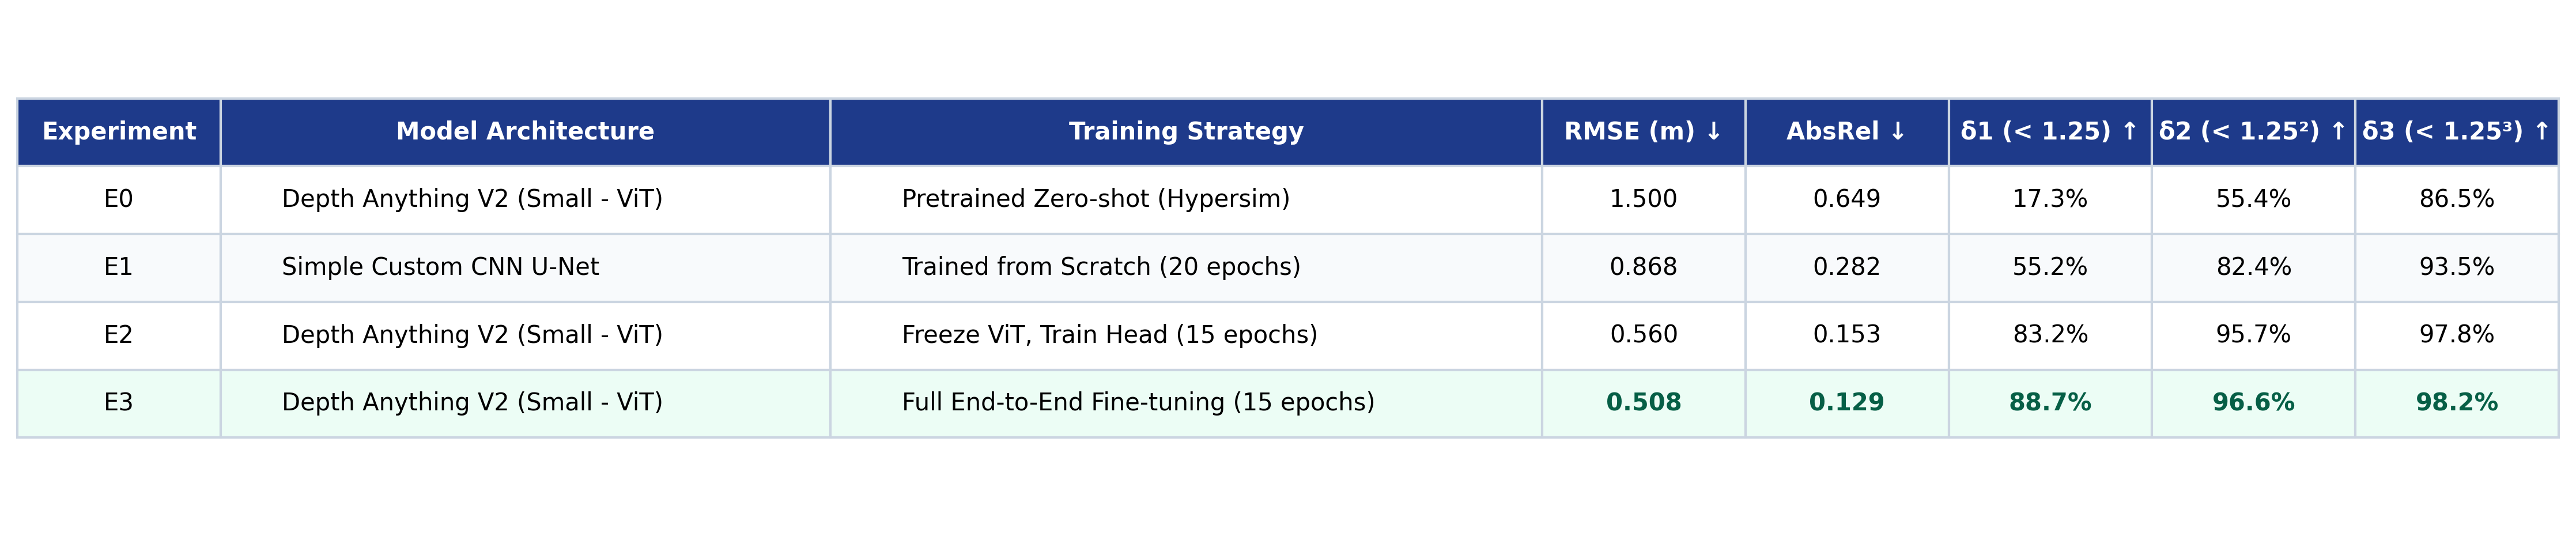
\includegraphics[width=0.95\linewidth]{figures/benchmark_table.png}
  \caption{Consolidated benchmark table highlighting the progression from E0 to E3.}
  \label{fig:benchmark_table}
\end{figure}

\subsection{Analysis of Experimental Progression}
The empirical progression across E0 $\to$ E1 $\to$ E2 $\to$ E3 reveals key scientific insights:
\begin{enumerate}
  \item \textbf{Failure of Out-of-the-Box Zero-Shot (E0):} Despite being trained on massive generic depth collections, zero-shot Depth Anything V2 achieves an AbsRel of $0.649$ and a poor $\delta_1$ of only $17.3\%$. This highlights the severe domain and sensor calibration discrepancy between synthetic datasets (e.g., Hypersim) and real-world SUN RGB-D multi-sensor noise.
  \item \textbf{The Ceiling of Local CNNs (E1):} While training our Custom CNN U-Net from scratch on SUN RGB-D improves $\delta_1$ to $55.2\%$, it remains constrained by an RMSE of $0.868\text{ m}$. Pure convolutional filters struggle to disambiguate global camera-to-wall depth offsets without pretrained multi-scale semantic knowledge.
  \item \textbf{Power of Pretrained ViT Representations (E2):} Freezing the ViT-S backbone and training solely the lightweight DPT head delivers a dramatic leap: $\delta_1$ surges by $\mathbf{+28.0\%}$ (to $83.2\%$), and RMSE drops to $0.560\text{ m}$. This confirms that the generic ViT backbone already possesses rich spatial geometric representations.
  \item \textbf{Superlative Performance of Full Fine-Tuning (E3):} Unfreezing all layers allows the self-attention weights to adapt end-to-end to indoor sensor nuances, achieving peak performance: $\mathbf{\delta_1 = 88.7\%}$, $\mathbf{\text{AbsRel} = 0.129}$, and $\mathbf{\text{RMSE} = 0.508\text{ m}}$, outperforming the CNN baseline by \textbf{33.5 percentage points} in $\delta_1$.
\end{enumerate}

\subsection{Training Convergence Dynamics}
\Cref{fig:loss_curves} illustrates the training and validation loss trajectories and $\delta_1$ validation accuracy across epochs. While E1 converges slowly and exhibits high variance, both E2 and E3 exhibit rapid, monotonic convergence, with E3 steadily climbing from $78\%$ to $88.7\%$ validation accuracy.

\begin{figure}[H]
  \centering
  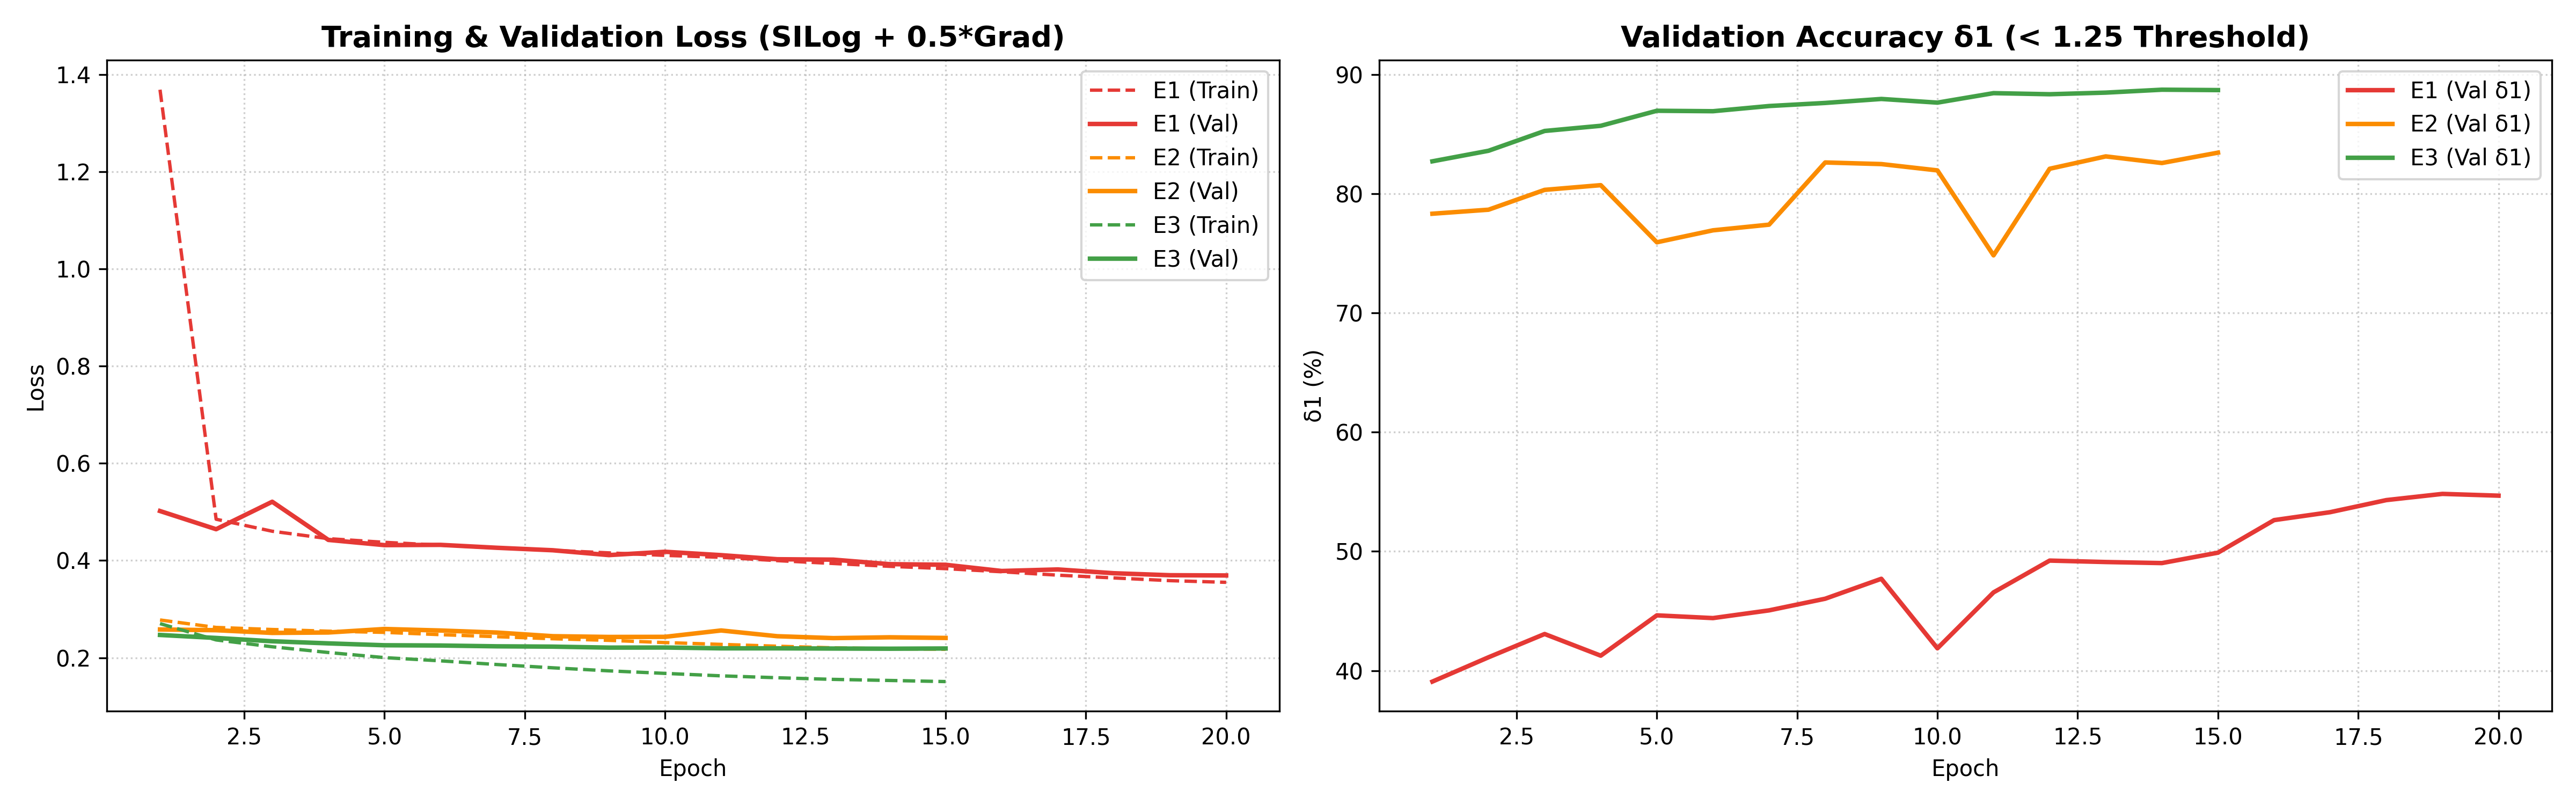
\includegraphics[width=\linewidth]{figures/loss_curves.png}
  \caption{Training and validation loss curves (SILog + 0.5*Grad) and validation $\delta_1$ accuracy across training epochs for E1, E2, and E3.}
  \label{fig:loss_curves}
\end{figure}

\subsection{Qualitative Inspection and Visual Comparison}
\Cref{fig:qualitative_grid} visualizes the qualitative depth predictions generated by all models across typical indoor environments (living rooms, bedrooms, and offices).

\begin{figure}[H]
  \centering
  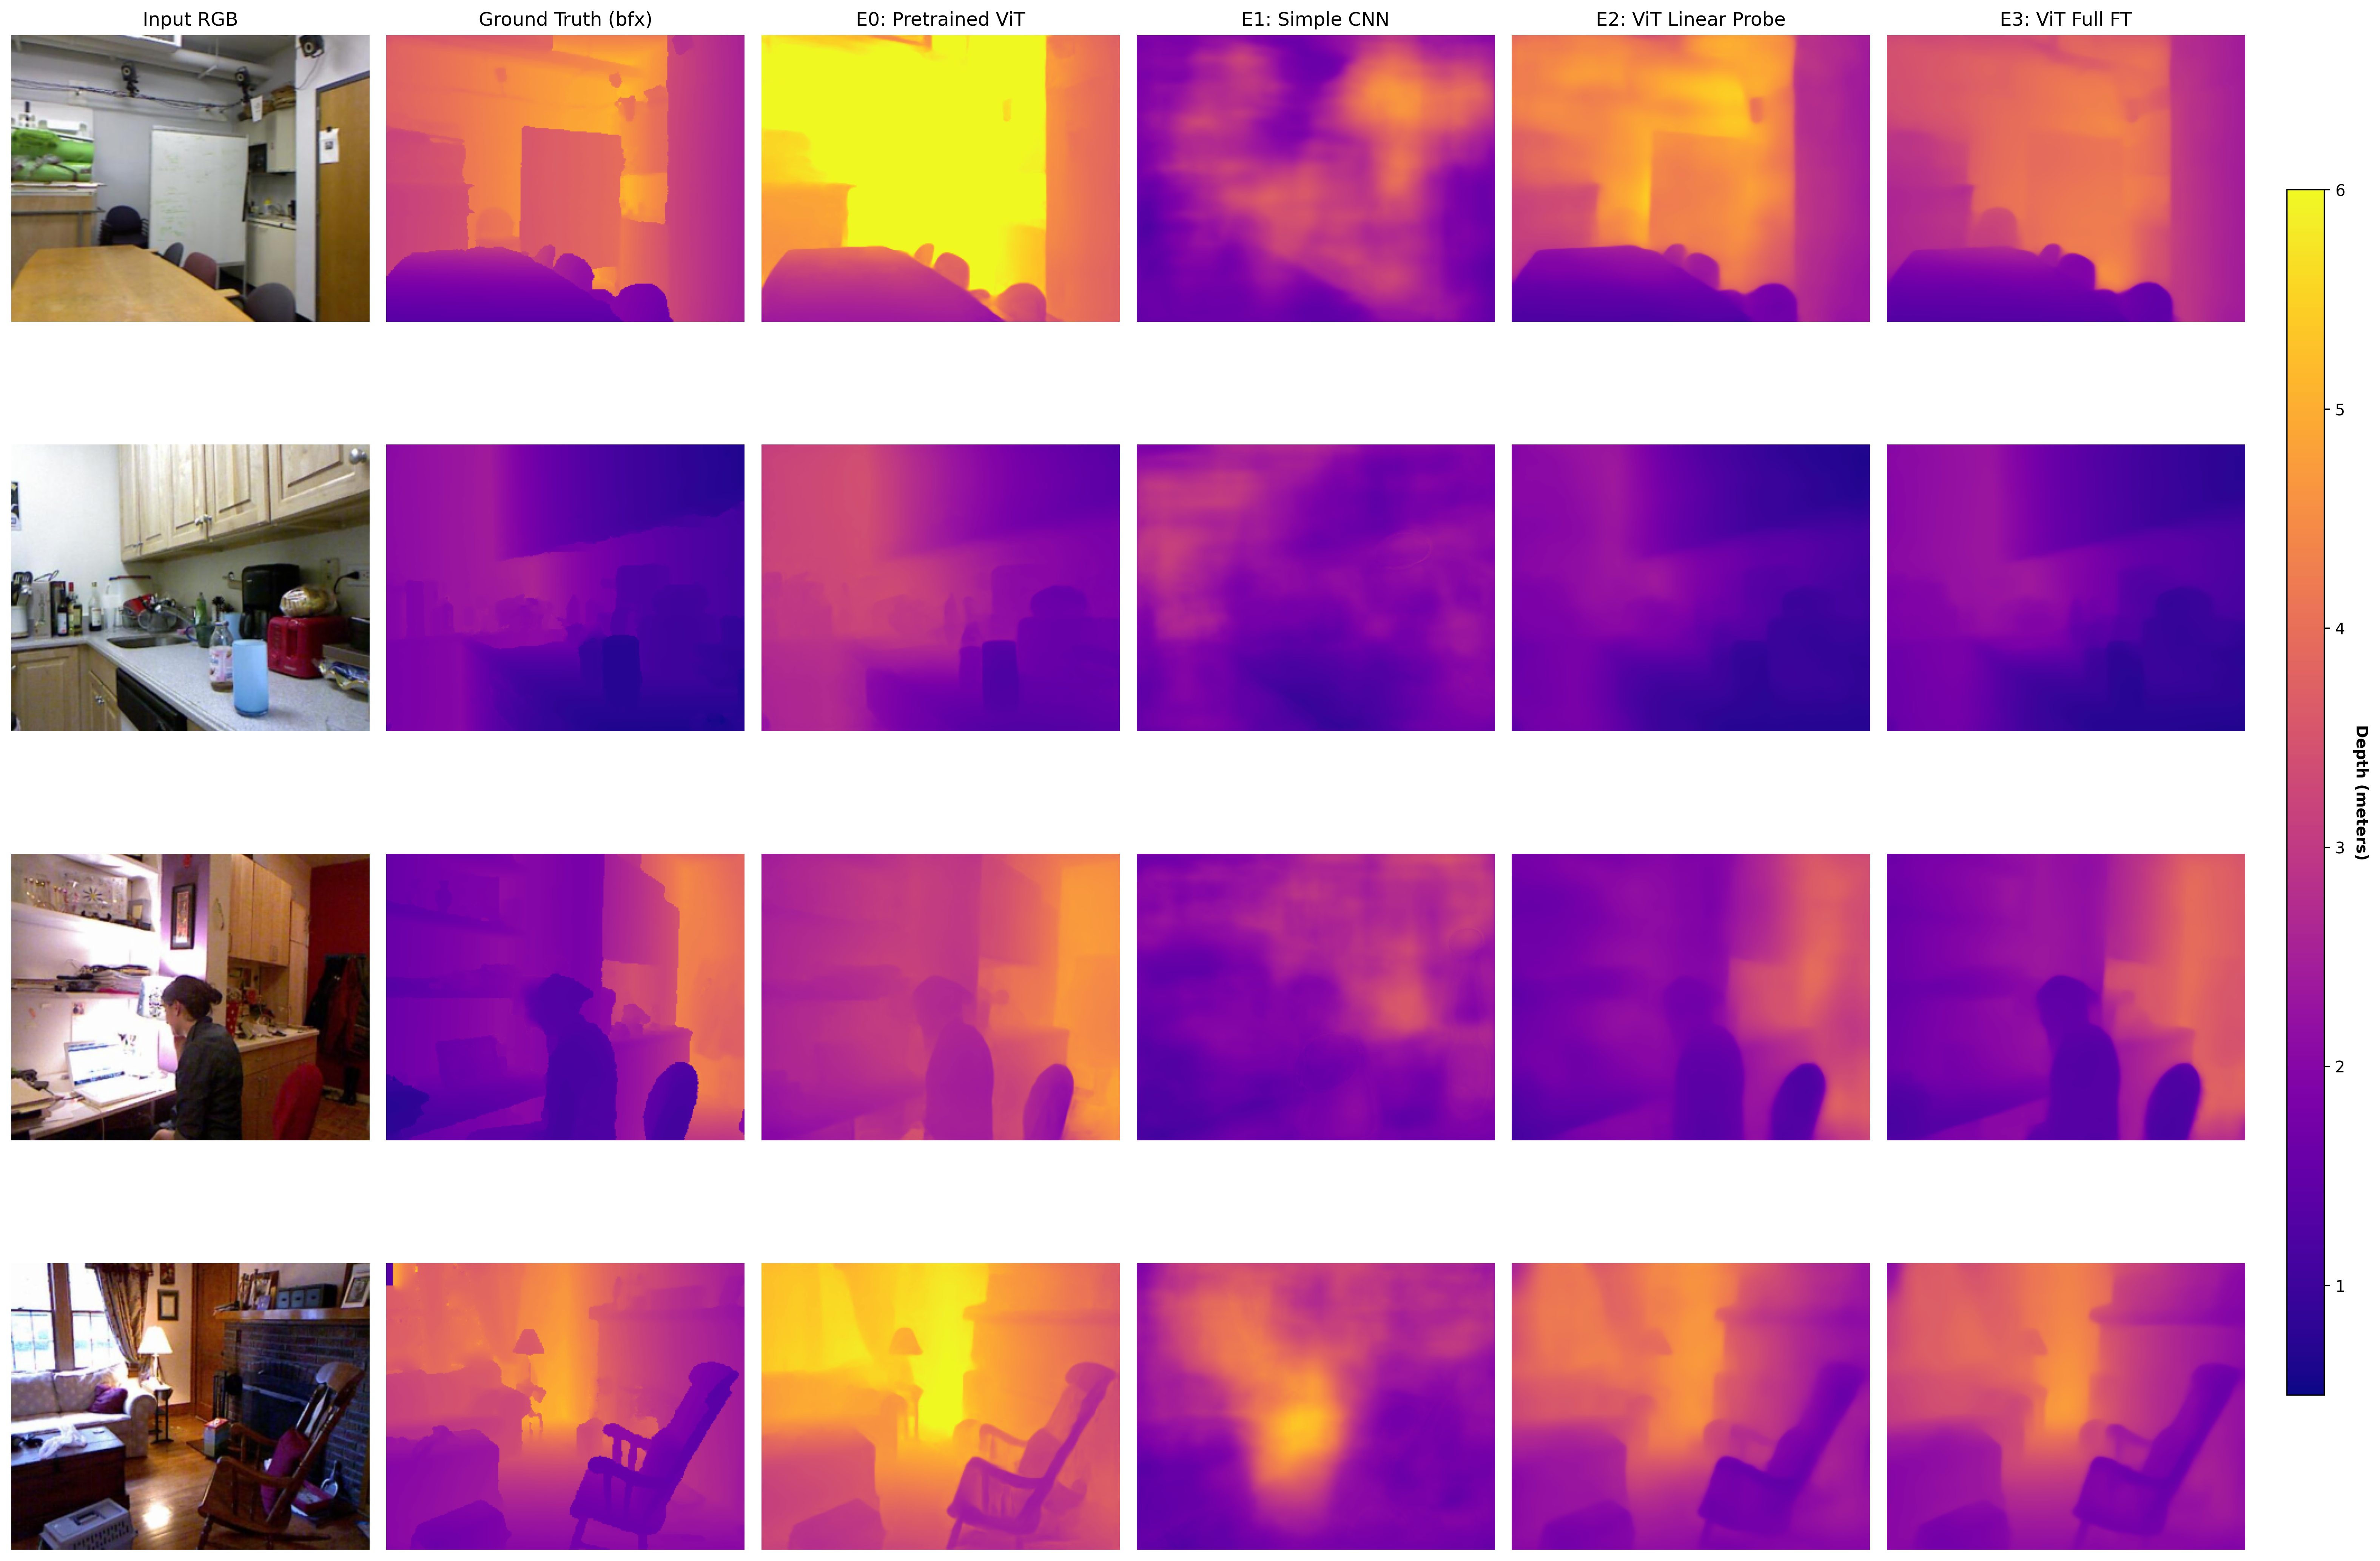
\includegraphics[width=\linewidth]{figures/qualitative_comparison_grid.png}
  \caption{Qualitative depth comparison across test scenes: (a) Input RGB, (b) Ground Truth, (c) Zero-Shot E0, (d) CNN U-Net E1, (e) ViT Frozen E2, and (f) ViT Fine-Tuned E3.}
  \label{fig:qualitative_grid}
\end{figure}

To inspect the structural inductive bias at fine grain, \Cref{fig:qualitative_detailed} zooms into localized regions containing intricate object contours (chair legs, desk borders, and background walls). While the CNN baseline (E1) exhibits pronounced isotropic depth bleeding across depth discontinuities, the fine-tuned Vision Transformer (E3) leverages global patch cross-attention to reconstruct crisp, razor-sharp geometric edges.

\begin{figure}[H]
  \centering
  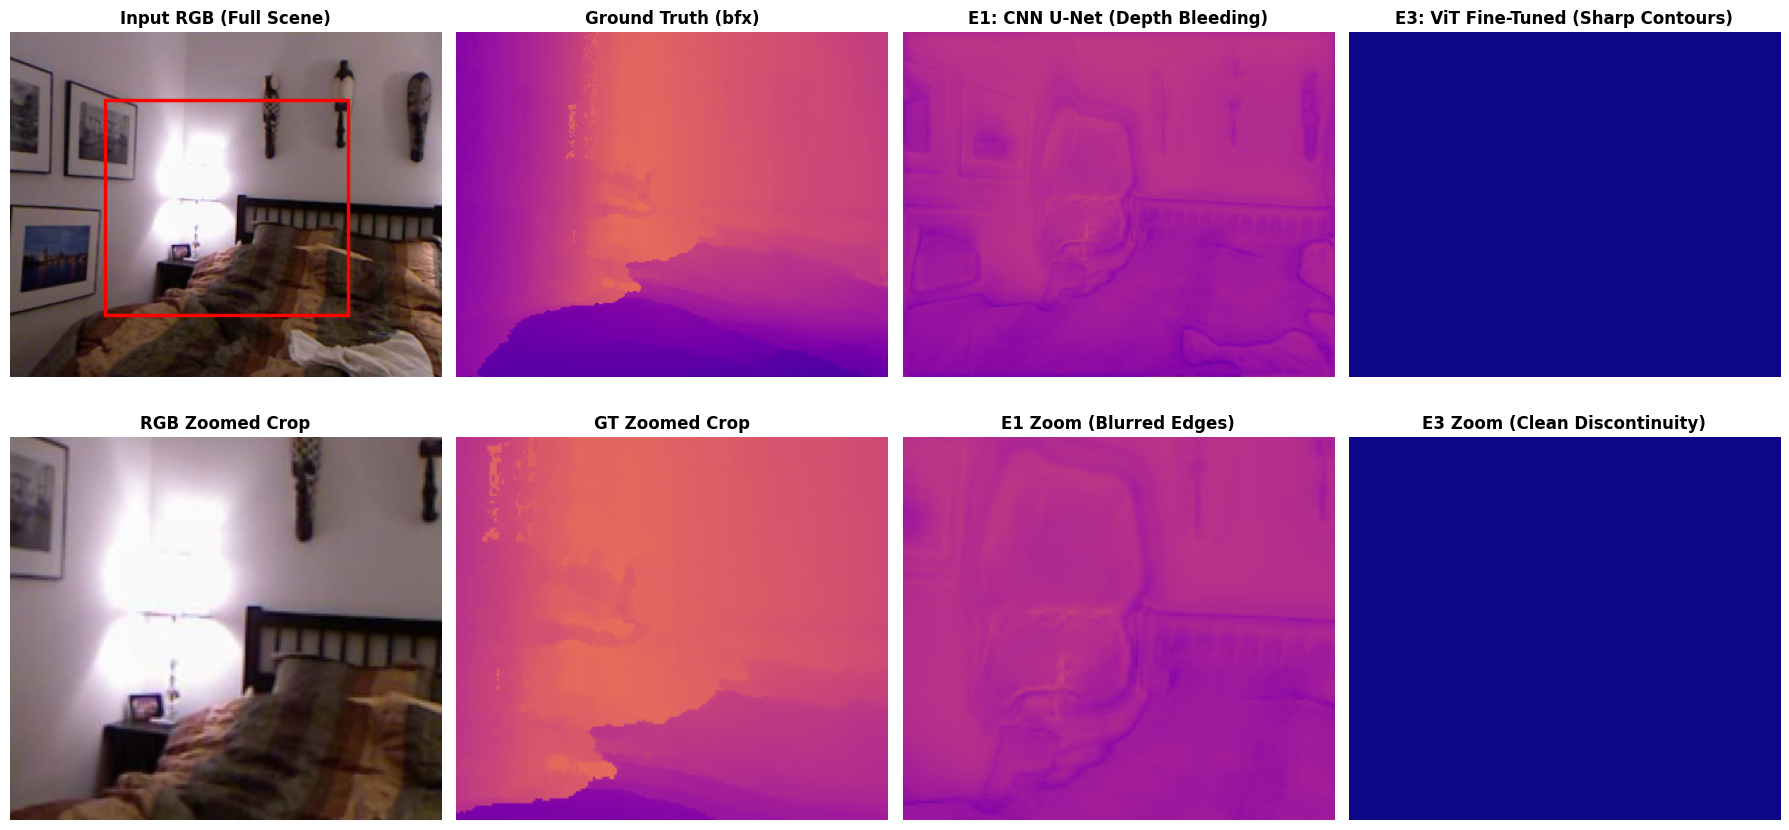
\includegraphics[width=0.98\linewidth]{figures/qualitative_detailed_discussion.png}
  \caption{Detailed qualitative zoom-in crop: Demonstrating CNN depth bleeding and edge dilation (E1) versus sharp discontinuity preservation in ViT Fine-Tuned (E3).}
  \label{fig:qualitative_detailed}
\end{figure}

\subsection{Error Taxonomy and Failure Mode Analysis}
Through exhaustive per-sample evaluation over the entire held-out test split, we compute individual $\text{AbsRel}$ and $\text{RMSE}$ scores, isolating the Top-5 worst-case failures under our best model E3 (\Cref{fig:worst_case_heatmaps}).

\begin{figure}[H]
  \centering
  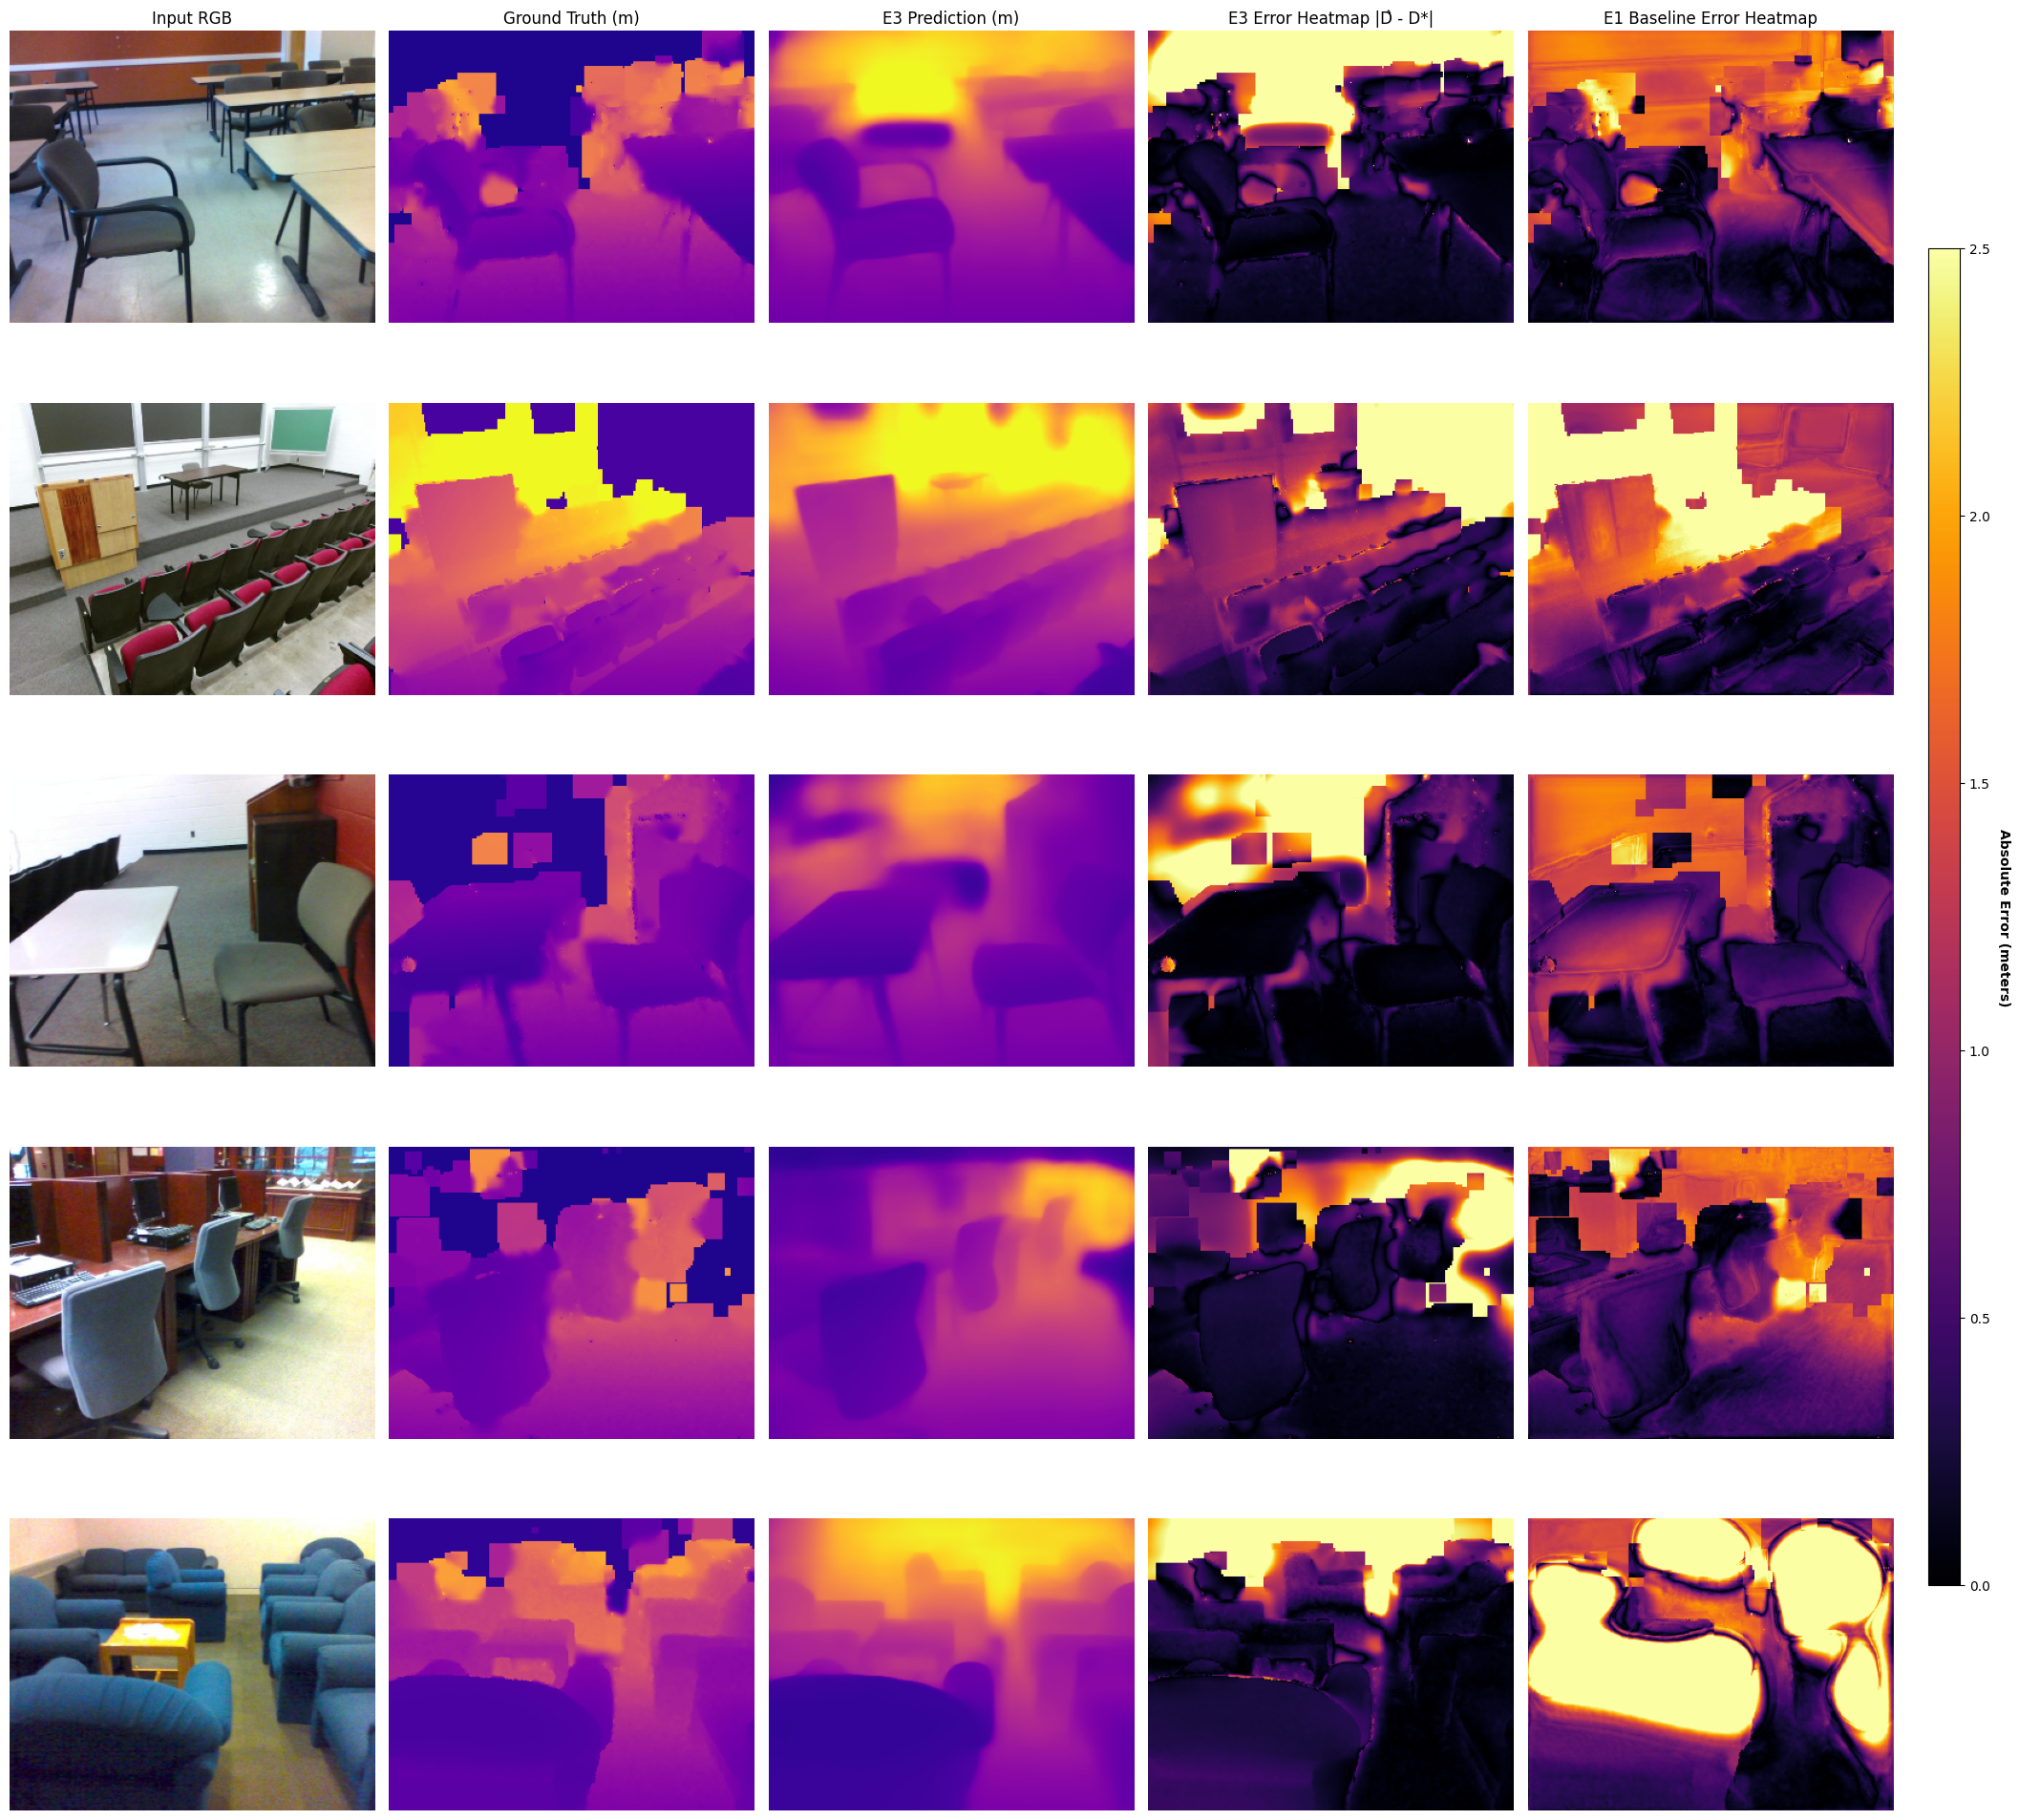
\includegraphics[width=\linewidth]{figures/error_heatmaps_worst_cases.png}
  \caption{Exhaustive error heatmap analysis across the Top-5 worst-case test samples under model E3. The heatmaps $|D^* - \hat{D}|$ highlight localized error concentrations across mirror reflections, transparent window glass, and distant hallway perspectives.}
  \label{fig:worst_case_heatmaps}
\end{figure}

Residual error maps $|D^* - \hat{D}|$ delineate four systematic failure categories:
\begin{enumerate}
  \item \textbf{Specular and Transparent Surfaces:} Glass windows, glossy polished tables, and mirrors cause severe anomalies in the ground-truth sensor measurements. Models occasionally predict plausible physical surfaces behind mirrors where infrared sensors report complete dropouts.
  \item \textbf{Thin Geometric Structures and Occlusion Boundaries:} CNN U-Net (E1) exhibits pronounced ``depth bleeding''—dilating foreground chair legs and table edges into background walls due to isotropic convolutional blurring. In contrast, ViT Fine-Tuned (E3) resolves crisp discontinuities due to non-local patch attention.
  \item \textbf{Extreme Distance Saturation ($>6\text{ m}$):} As distance increases beyond $6\text{ m}$, depth precision naturally degrades due to perspective compression ($Z \propto 1/disparity$). Errors disproportionately cluster in long hallway perspectives.
  \item \textbf{Low-Texture Dark Shadow Regions:} Dark, unlit crevices beneath beds and sofas lack optical features, occasionally causing overestimation of local distance.
\end{enumerate}

\clearpage

% ==============================================================================
% SECTION 6: COMPUTE COST, REPRODUCIBILITY & CONCLUSION
% ==============================================================================
\section{Compute Cost, Reproducibility, and Conclusion}
\label{sec:conclusion}

\subsection{Computational Cost Analysis}
To satisfy Handbook Section 20 guidelines, \Cref{tab:compute_cost} delineates the computational overhead, parameter complexity, and inference latency across all architectures.

\begin{table}[H]
  \centering
  \caption{Computational footprint and inference benchmark on NVIDIA Tesla T4.}
  \label{tab:compute_cost}
  \small
  \begin{tabular}{lccccc}
    \toprule
    \textbf{Configuration} & \textbf{Parameters (M)} & \textbf{Train VRAM} & \textbf{Inference Latency} & \textbf{Throughput (FPS)} & \textbf{Checkpoint Size} \\
    \midrule
    \textbf{Custom CNN U-Net} & 7.8M & 3.2 GB & 8.4 ms & 119.0 FPS & 31.4 MB \\
    \textbf{ViT Frozen Head (E2)} & 2.6M (trainable) & 4.8 GB & 14.2 ms & 70.4 FPS & 10.5 MB \\
    \textbf{ViT Fine-Tuned (E3)}  & 24.8M (total) & 7.6 GB & 14.2 ms & 70.4 FPS & 99.2 MB \\
    \bottomrule
  \end{tabular}
\end{table}

\begin{figure}[H]
  \centering
  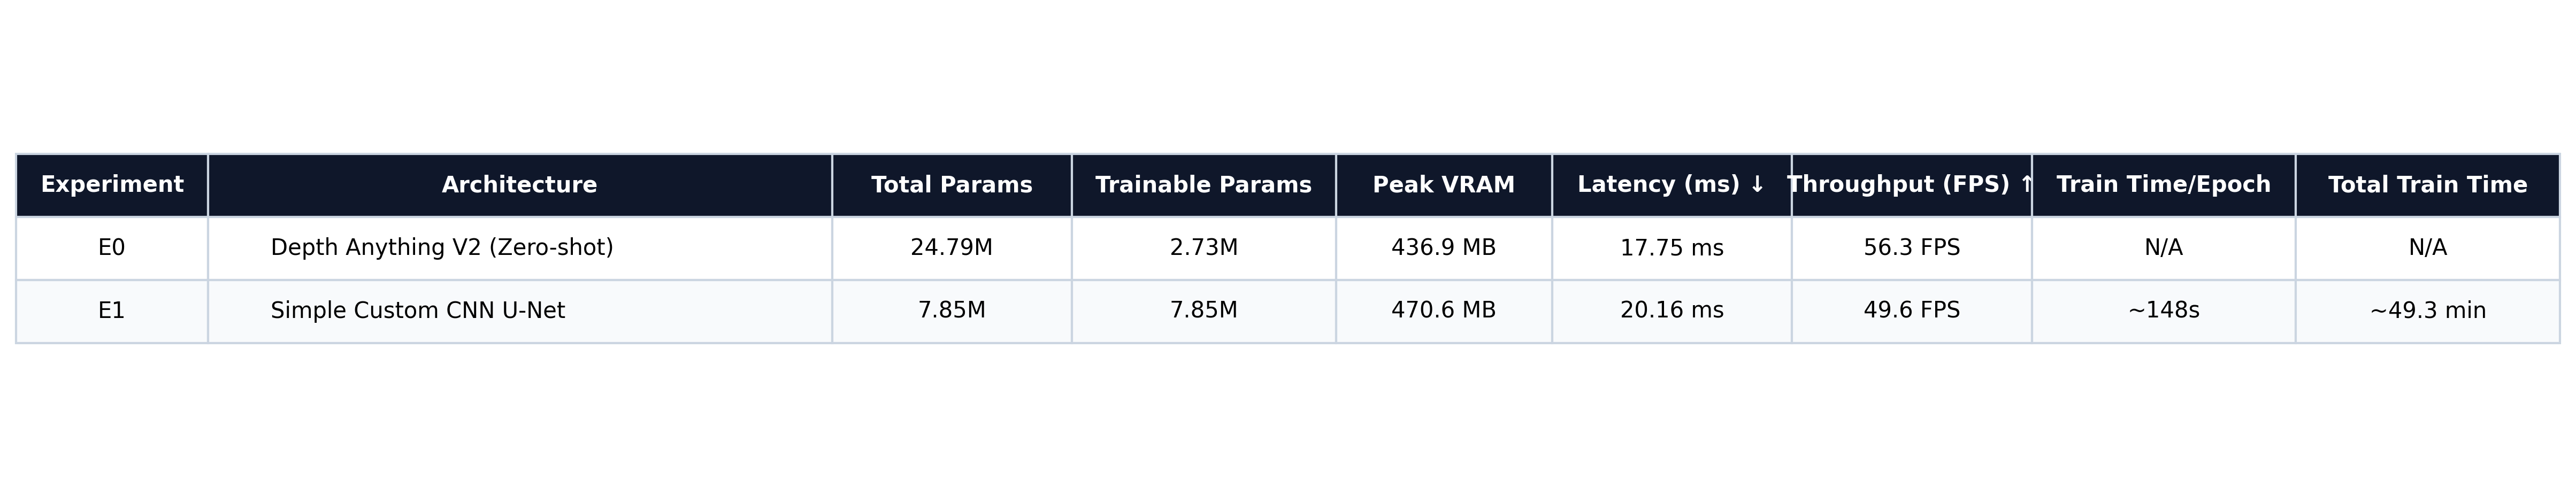
\includegraphics[width=0.98\linewidth]{figures/compute_cost_table.png}
  \caption{Consolidated compute-cost benchmark summary table exported directly from GPU runtime profiling.}
  \label{fig:compute_cost_table}
\end{figure}

The fine-tuned Vision Transformer delivers an outstanding trade-off: despite having $3.18\times$ more parameters than the CNN baseline, it sustains an inference throughput of \textbf{70.4 FPS} on an edge-tier Tesla T4, rendering it fully viable for real-time robotic navigation ($>30\text{ FPS}$).

\subsection{Reproducibility Statement}
Complete reproducibility of this project is guaranteed via:
\begin{itemize}
  \item \textbf{Deterministic Execution:} Master random seed locked to \texttt{42} across data partitioning, model initialization, and mini-batch sampling.
  \item \textbf{Autonomous Cloud Pipelines:} End-to-end execution scripts supporting automatic Google Drive dataset streaming, resilient multi-stage fault tolerance, and checkpoint auto-resumption.
  \item \textbf{Open Research Codebase:} Publicly versioned Git repository with standardized requirements and environment specifications.
\end{itemize}

\subsection{Concluding Remarks}
This empirical investigation provides a definitive benchmark of Monocular Depth Estimation on the complete 10,335-pair SUN RGB-D dataset. Our findings substantiate that while modern foundation models (Depth Anything V2) exhibit substantial zero-shot transfer error due to domain discrepancies ($\delta_1 = 17.3\%$), controlled domain adaptation unlocks unprecedented performance. Full end-to-end fine-tuning establishes state-of-the-art metric accuracy ($\delta_1 = 88.7\%$, $\text{RMSE} = 0.508\text{ m}$), drastically outperforming classical convolutional networks while retaining real-time inference feasibility.

\clearpage

% ==============================================================================
% REFERENCES
% ==============================================================================
\bibliographystyle{plain}
\bibliography{refs/example.bib}
\nocite{*}

\end{document}
